\documentclass[12pt,letterpaper]{article}
\usepackage{graphicx,textcomp}
\usepackage{natbib}
\usepackage{setspace}
\usepackage{fullpage}
\usepackage{color}
\usepackage[reqno]{amsmath}
\usepackage{amsthm}
\usepackage{fancyvrb}
\usepackage{amssymb,enumerate}
\usepackage[all]{xy}
\usepackage{endnotes}
\usepackage{lscape}
\newtheorem{com}{Comment}
\usepackage{float}
\usepackage{hyperref}
\newtheorem{lem} {Lemma}
\newtheorem{prop}{Proposition}
\newtheorem{thm}{Theorem}
\newtheorem{defn}{Definition}
\newtheorem{cor}{Corollary}
\newtheorem{obs}{Observation}
\usepackage[compact]{titlesec}
\usepackage{dcolumn}
\usepackage{tikz}
\usetikzlibrary{arrows}
\usepackage{multirow}
\usepackage{xcolor}
\newcolumntype{.}{D{.}{.}{-1}}
\newcolumntype{d}[1]{D{.}{.}{#1}}
\definecolor{light-gray}{gray}{0.65}
\usepackage{url}
\usepackage{listings}
\usepackage{color}
\usepackage{amsthm}
\newtheorem{hypothesis}{Hypothesis}

\usepackage{booktabs}
\usepackage{dcolumn}
\usepackage{longtable}

% --- Listings Style Update ---
\definecolor{codegreen}{rgb}{0,0.6,0}
\definecolor{backcolour}{rgb}{0.95,0.95,0.92}

\lstdefinestyle{mystyle}{
	commentstyle=\color{codegreen},
	keywordstyle=\color{blue},
	stringstyle=\color{codegreen},
	backgroundcolor=\color{backcolour},
	basicstyle=\ttfamily\footnotesize,
	breaklines=true,
	captionpos=b,
	keepspaces=true,
	numbers=left,
	numbersep=5pt,
	showspaces=false,
	showstringspaces=false,
	showtabs=false,
	tabsize=2
}
\lstset{style=mystyle}
% -----------------------------

\newcommand{\Sref}[1]{Section~\ref{#1}}
\newtheorem{hyp}{Hypothesis}

\begin{document}
	
	% Title Page
	\begin{titlepage}
		\centering
		\vspace*{2cm}
		{\LARGE \textbf{Why Do States Abandon the Inheritance Tax? \\
				The Role of Revenue Efficiency and Democratic Institutions} \par}
		\vspace{1cm}
		{\Large \textbf{Applied Statistical Analysis II} \par}
		\vspace{1cm}
		{\large \textbf{Sein Kim (25358755)} \par}
		\vfill
		{\large \textbf{Date of submission: 30/03/2026 (Mon)} \par}
		\vfill
		\begin{center}
			\small
			I have read and understood the plagiarism provisions in the General Regulations of the University Calendar for the current year, found at \url{http://www.tcd.ie/calendar}. \\
			\vspace{0.3cm}
			I have also read and understood the guide, and completed the ‘Ready Steady Write’ Tutorial on avoiding plagiarism, located at \url{https://libguides.tcd.ie/academic-integrity/ready-steady-write}.
		\end{center}
		\vspace{1cm}
		
\includegraphics[width=0.6\textwidth]{TCD_logo.jpg} \\ 
		\vspace{0.5cm}
		{\large \textbf{Trinity College Dublin} \par}
		\smallskip
		{\large \textbf{MSc Applied Social Data Science} \par}
		\vfill
		\vspace*{1cm}
	\end{titlepage}
	
	\newpage
	{\setstretch{2} \tableofcontents}
	\newpage
	
	\section{Original Study}
	\noindent I replicate the following study: "Genschel, P., Limberg, J., \& Seelkopf, L. (2024). Revenue, Redistribution, and the Rise and Fall of Inheritance Taxation. Comparative Political Studies, 57(9), 1475-1505." 

\vspace{0.3cm}
	
	\subsection{Background and Research Question}
	\begin{itemize}
		\item \textbf{Research Question:} Why do many countries repeal the inheritance tax after having previously introduced it? 
		\item \textbf{Limitations of Existing Literature:} Conventional public policy research holds that policies are rarely terminated due to entrenched interests. However, inheritance taxation is an exception, showing a rapid decline since the 1960s.
		\item \textbf{Authors' Perspective:} The "rise and fall" of the inheritance tax is determined by changes in its revenue function for the state, rather than just democratic pressure or elite capture.
	\end{itemize}
	
	\subsection{Hypotheses}
	\begin{itemize}
		\item \textbf{Revenue Hypothesis:} The likelihood of inheritance tax repeal increases as governments adopt and expand more efficient revenue instruments, such as income taxes and Value Added Tax (VAT).
		\item \textbf{Redistribution Hypothesis:} Once fiscal purpose weakens, the survival of the tax depends on redistributive features; therefore, non-democratic governments are more likely to repeal the tax than democracies.
	\end{itemize}
	
	\subsection{Data and Method}
	\begin{itemize}
		\item \textbf{Data:} The authors use a novel dataset tracking inheritance tax introductions and repeals for a global sample of 87 countries over approximately two centuries (1759–2015).
		\item \textbf{Method:} The study utilizes a Binary Time-Series Cross-Section (BTSCS) dataset.
		\item \textbf{Model:} 	The analysis is conducted using Logit Models with a cubic polynomial approximation $(t,t^2,t^3)$ to account for temporal dependence and analyze repeal risk.
	\end{itemize}
	\begin{figure}[H]\centering
		\caption{Inheritance Tax Introductions and Repeals over Time}
		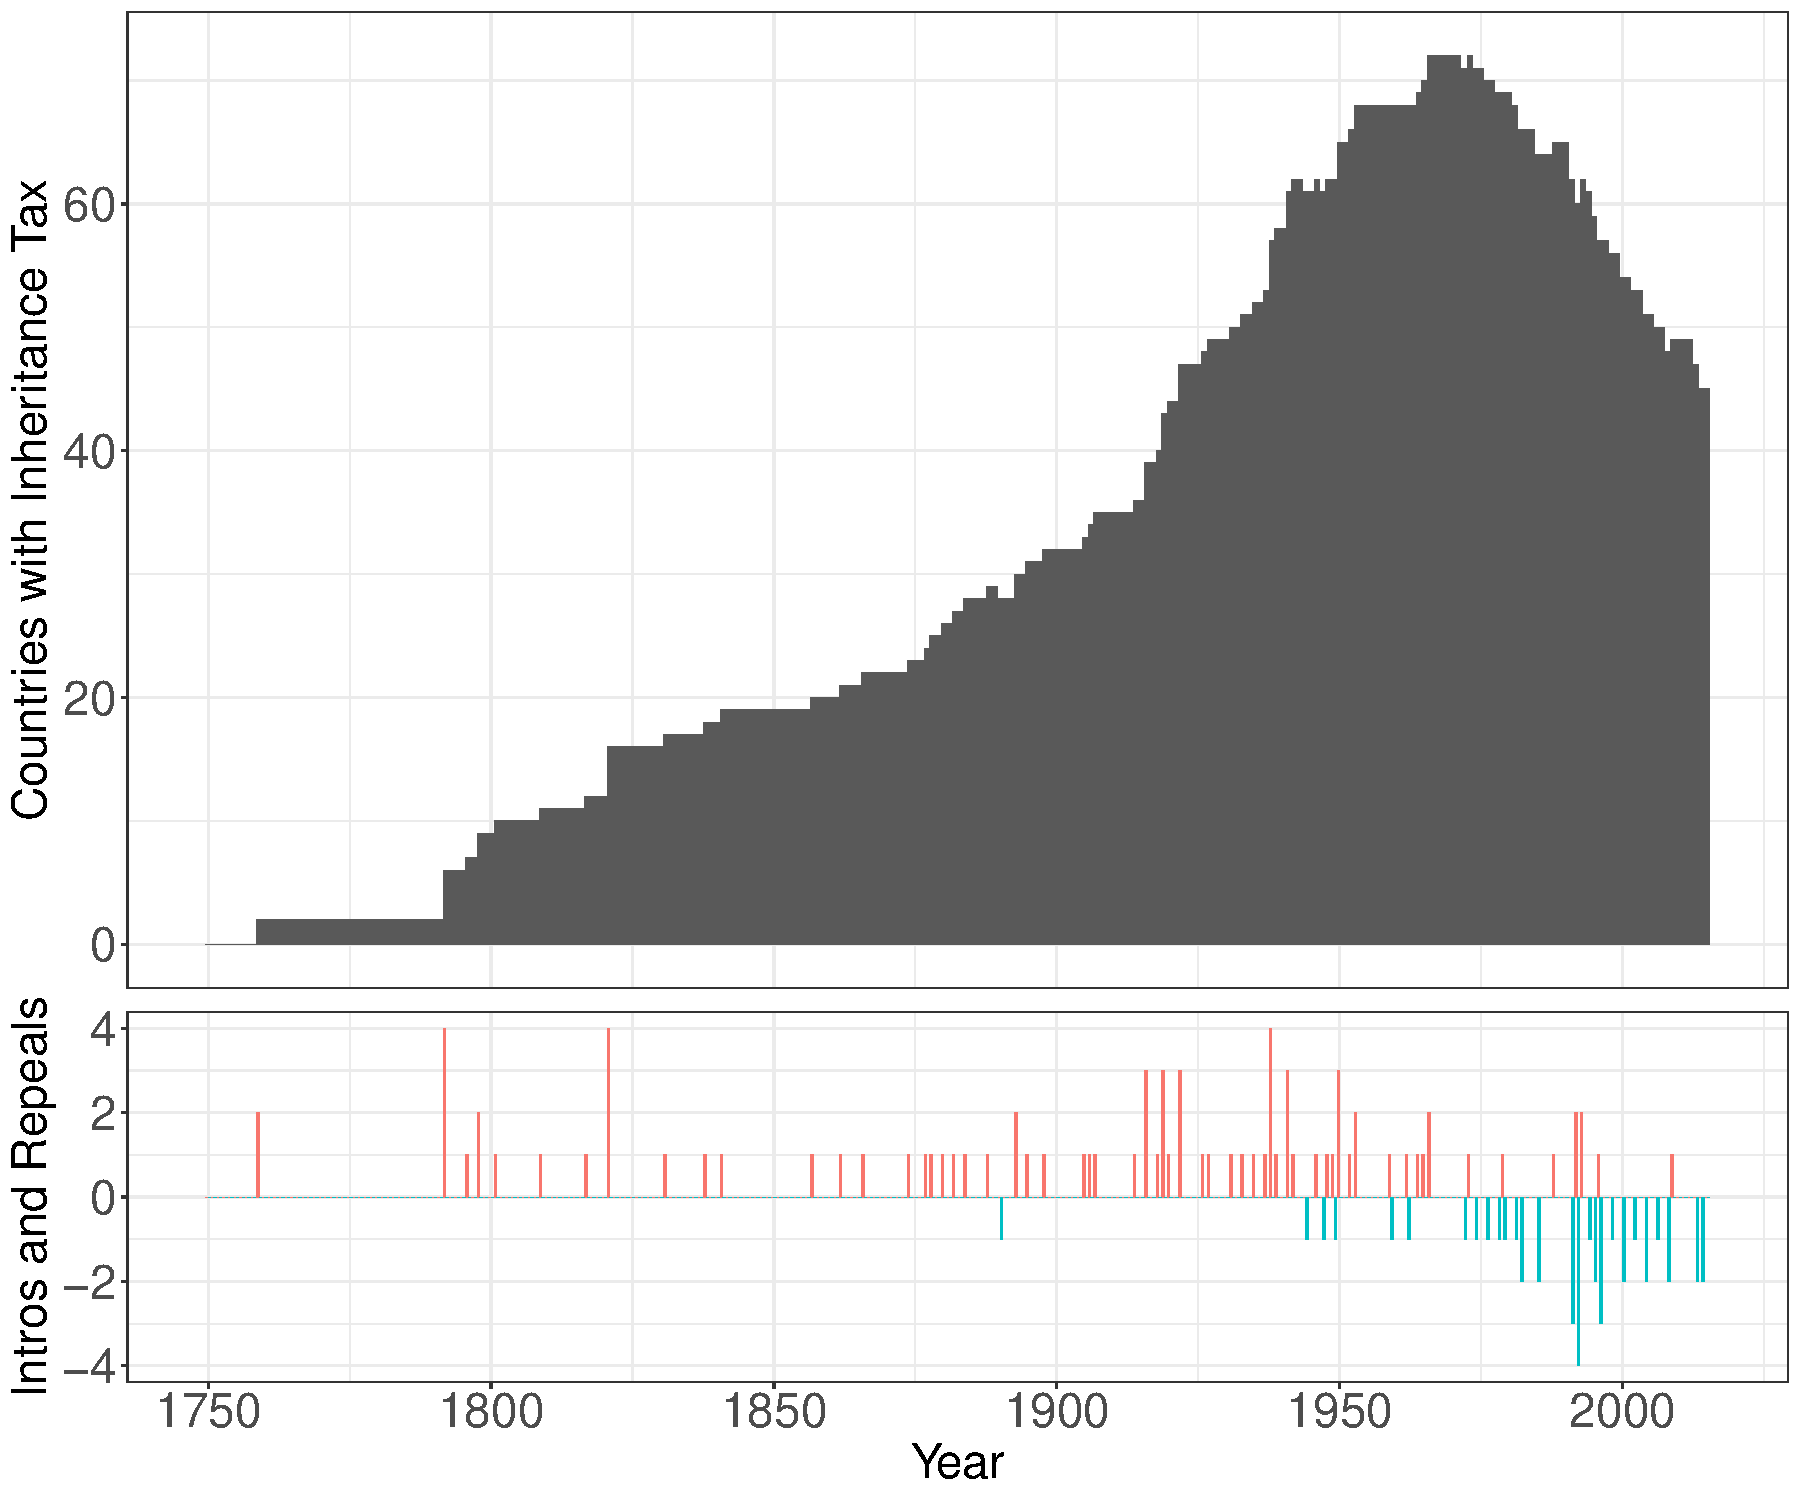
\includegraphics[width=1.0\textwidth]{data_SK/Figure1.pdf}
	\end{figure}
	\textbf{Figure 1 Description: }The number of countries levying an inheritance tax increased steeply during the 19th and early 20th centuries but has declined rapidly since the 1960s as repeals began to outpace introductions.
	
\newpage
	\section{Data}
	\noindent The main analysis is conducted using the \texttt{merge\_full\_2} dataset, which is a Binary Time-Series Cross-Section (BTSCS) dataset tracking countries at risk of repealing their inheritance tax.
	\vspace{0.3cm}
	\subsection{Outcome Variable}
	\noindent Inheritance tax repeal (y), coded as:
	\begin{itemize}
		\item Inheritance tax is permanently repealed: 1
		\item Inheritance tax is maintained (or censored): 0
	\end{itemize}
		\vspace{0.3cm}
	\subsection{Input Variables}
	\subsubsection{Key Independent Variables:}
	\begin{itemize}
		\item \textbf{Major modern taxes (other\_tax):} An index measuring the introduction of income and consumption taxes, coded as 0 (neither), 1 (either), or 2 (both).
		\item \textbf{Democracy (democracy):} A binary indicator of democratic regime type.
	\end{itemize}
	
	\subsubsection{Control Variables:}
	\begin{itemize}
		\item \textbf{Fiscal/Economic:} Includes indicators for recent war (war\_previous), recent economic recession (recession\_prev\_5), and social policy introduction (wfs\_intro\_previous).
		\item \textbf{Demographic/Structural:} Includes logged population for tax competition \texttt{(log(population\_new)}, logged GDP per capita \texttt{(log\_gdp\_cap)}, life expectancy \texttt{(e\_pelifeex)}, and logged time since the tax was introduced \texttt{(log(time\_since\_intro))}.
		\item \textbf{Temporal Dependence ($t, t2, t3$): }A cubic polynomial approximation of time at risk to account for temporal dependence in the BTSCS data.
	\end{itemize}
	
	\newpage
	\section{Original Model}
	\noindent The authors build their argument by first exploring the historical conditions of the inheritance tax's introduction and consolidation, followed by a logistic regression model to analyze the determinants of its repeal.
		\vspace{0.3cm}
	\subsection{Historical Context (Figures 2, 3, and 4)}
	\noindent Before testing the repeal of the inheritance tax, the authors illustrate why it was introduced in the first place. Figure 2 shows that introductions were closely associated with spending-intensive events like wars, recessions, and the introduction of social policies. Figure 3 demonstrates that inheritance taxes were mostly adopted before other modern taxes (income and consumption taxes), highlighting their crucial role when alternative revenues were scarce.
	The R code snippet to replicate Figure 3 is as follows:
	
	
	\begin{lstlisting}[language=R]
		fig3 <- rank_inheritance %>%
		ggplot(., aes(x=rank_tax_base, fill =rank_tax_base )) +
		geom_bar(aes(y = after_stat(count)/sum(after_stat(count)))) + 
		scale_y_continuous(labels=scales::percent) +
		theme_bw() +
		ylab("Share of Countries") + 
		scale_fill_grey() +
		xlab("Historical Timing Inheritance Tax") +
		theme(text = element_text(size=20),
		legend.position = "none",
		axis.text.x = element_text(angle = 45, vjust = 1, hjust=1))\end{lstlisting}
	
	\begin{figure}[H]
		\centering
		\begin{minipage}{0.45\textwidth}
			\centering
			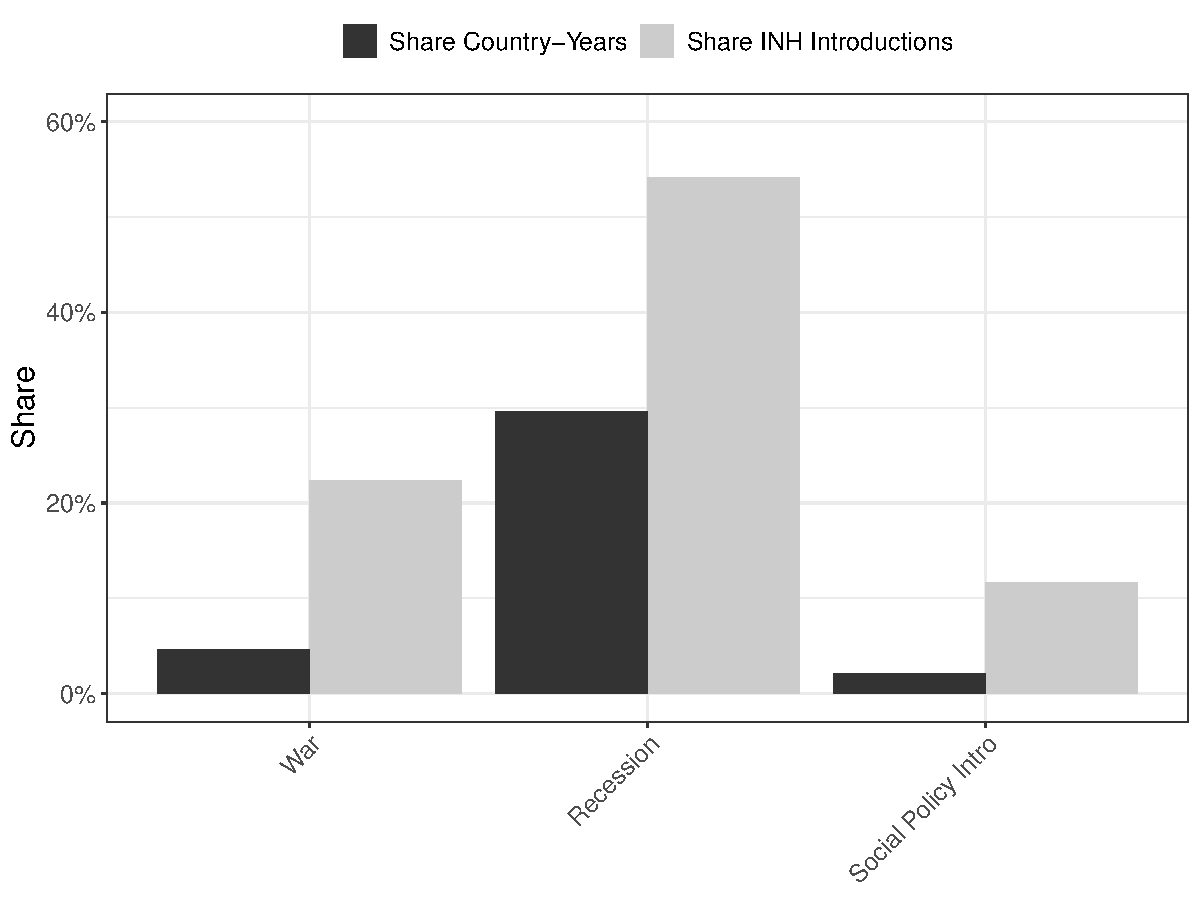
\includegraphics[width=\textwidth]{data_SK/Figure2.pdf}
			\caption{Context of Introductions}
		\end{minipage}
		\hfill
		\begin{minipage}{0.45\textwidth}
			\centering
			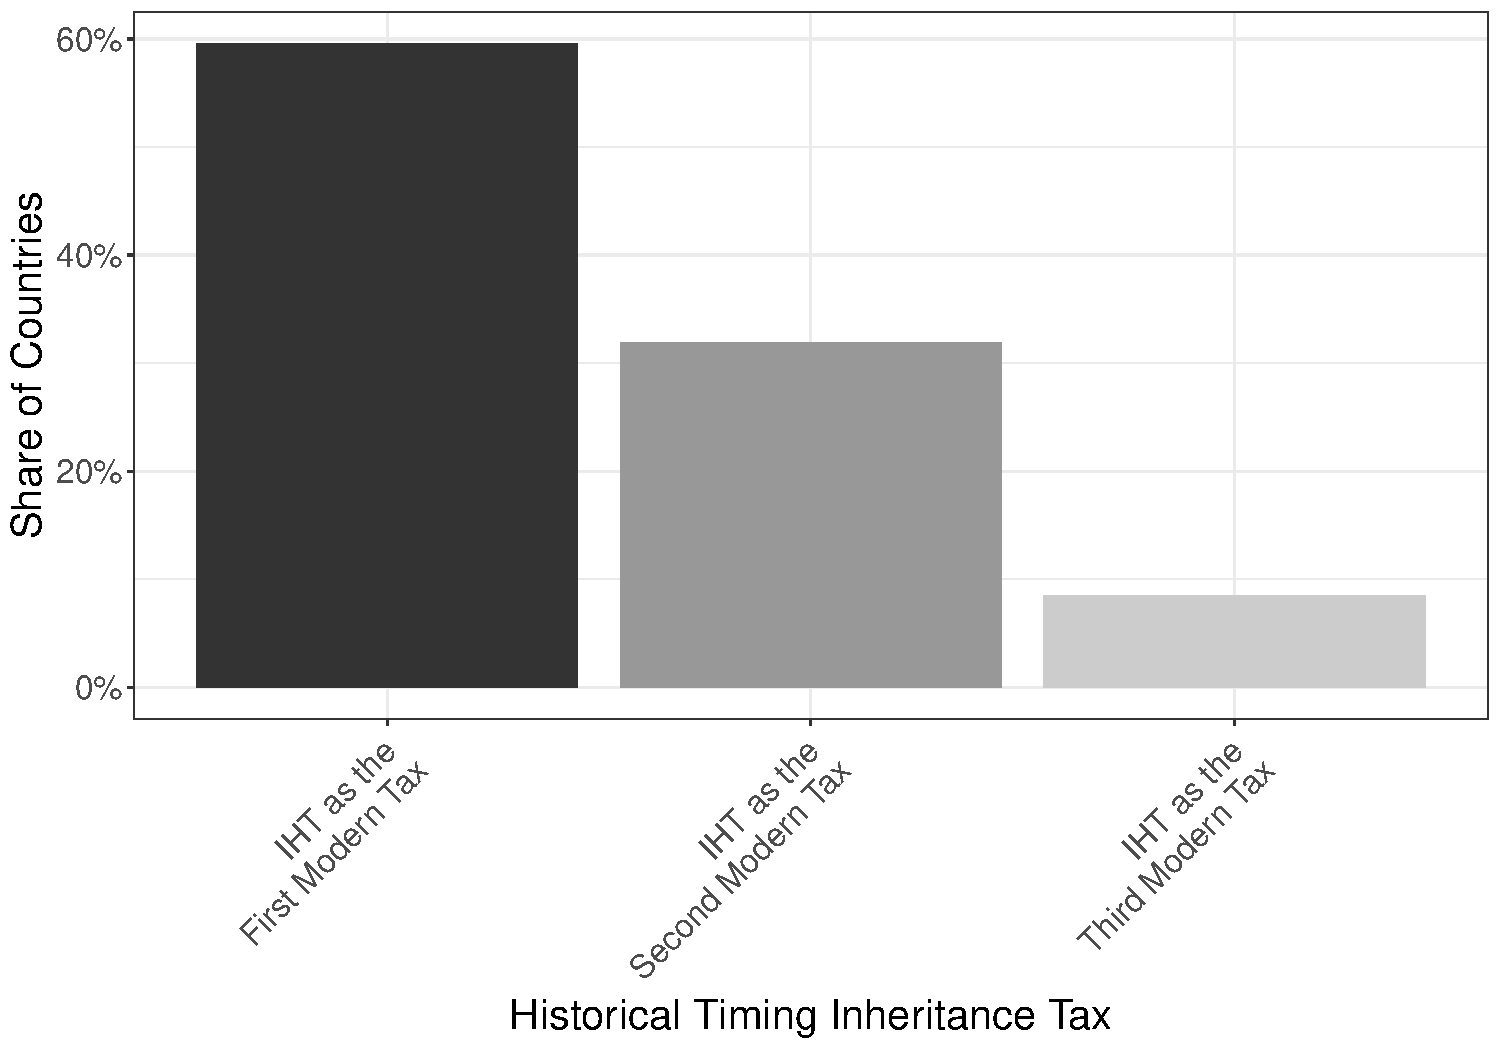
\includegraphics[width=\textwidth]{data_SK/Figure3.pdf}
			\caption{Timing of IHT}
		\end{minipage}
	\end{figure}
	\noindent However, as other efficient revenue instruments were developed, the fiscal significance of the inheritance tax declined. Figure 4 uses Austria as a case study to show how the inheritance tax revenue as a percentage of total revenue steadily dropped over the 20th century.
	
		\begin{figure}[H]\centering
		\caption{}
		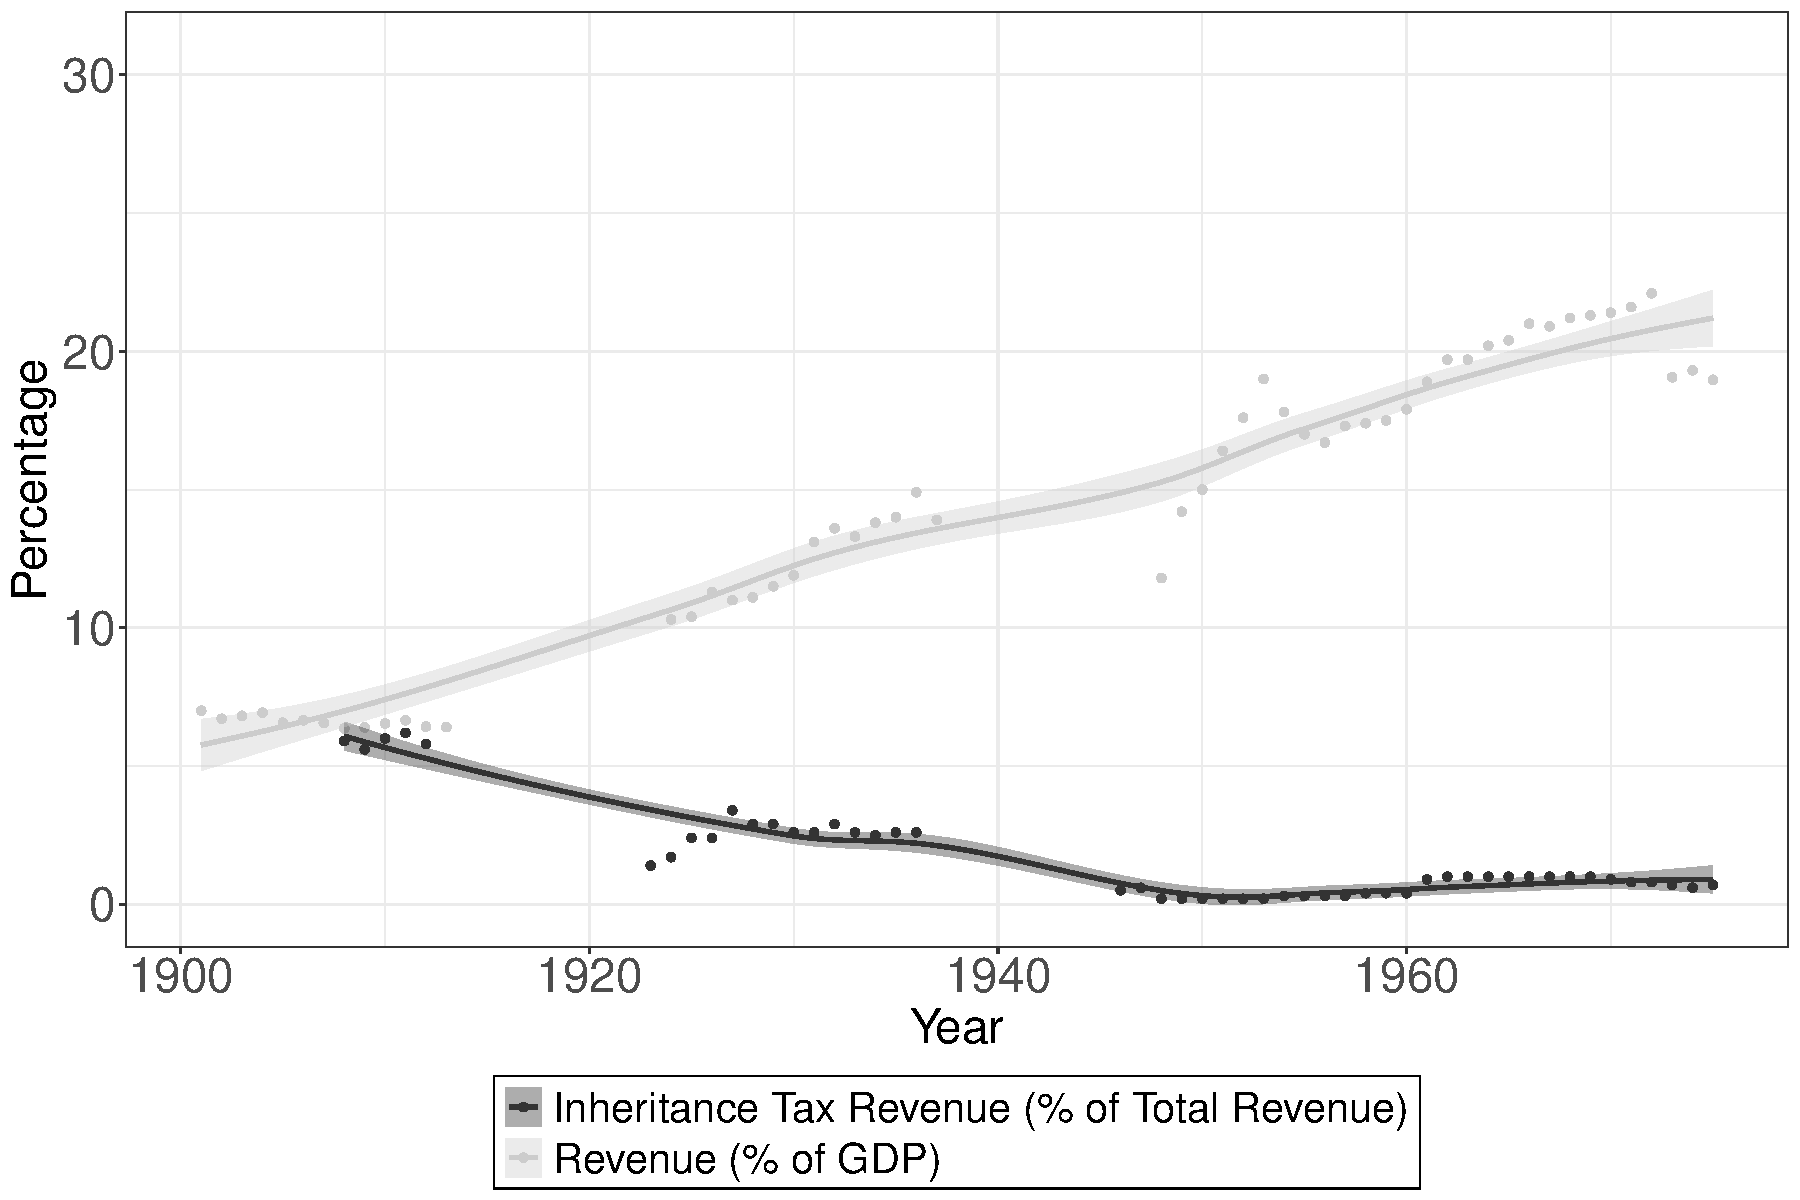
\includegraphics[width=0.7\textwidth]{data_SK/Figure4.pdf}
	\end{figure}
	\subsection{Main Regression Model (Table 1)}
	To test their hypotheses on tax repeal, the authors run a logistic regression model with a maximum likelihood estimation technique. To account for temporal dependence in the Binary Time-Series Cross-Section (BTSCS) data, they include a cubic polynomial approximation (t, t2, t3).
	The R code to replicate the fully specified model (Model 3) is as follows:

	\begin{lstlisting}[language=R]
		main_inh_3 <- glm(y ~ other_tax + democracy  + 
		war_previous + recession_prev_5 + wfs_intro_previous +
		log(time_since_intro) + log_gdp_cap + e_pelifeex + log(population_new) + t + t2 + t3,
		data = merge_full_2, family=binomial(link="logit")))\end{lstlisting}
	
	\begin{center}
\begin{small}
\begin{longtable}{l@{} D{.}{.}{4.6}@{} D{.}{.}{4.6}@{} D{.}{.}{4.6}@{}}
\caption{Regression Results for Inheritance Tax Repeal}
\label{table:coefficients}\\
\toprule
 & \multicolumn{1}{c}{Model 1} & \multicolumn{1}{c}{Model 2} & \multicolumn{1}{c}{Model 3} \\
\midrule
\endfirsthead
\toprule
 & \multicolumn{1}{c}{Model 1} & \multicolumn{1}{c}{Model 2} & \multicolumn{1}{c}{Model 3} \\
\midrule
\endhead
\bottomrule
\endfoot
\bottomrule
\multicolumn{4}{l}{\tiny{$^{***}p<0.01$; $^{**}p<0.05$; $^{*}p<0.1$}}\\
\endlastfoot
Major Modern Taxes               & 1.576^{***} & 1.546^{***} & 1.098^{**}   \\
                                 & (0.418)     & (0.417)     & (0.453)      \\
Democracy                        & -0.779^{**} & -0.763^{**} & -1.197^{***} \\
                                 & (0.356)     & (0.359)     & (0.387)      \\
War                              &             & 0.199       & 0.764        \\
                                 &             & (1.032)     & (1.066)      \\
Recession                        &             & 0.266       & 0.384        \\
                                 &             & (0.355)     & (0.356)      \\
Social Policy Intro              &             & -15.602     & -15.311      \\
                                 &             & (570.644)   & (568.308)    \\
Tax Competition (Population log) &             &             & 0.034        \\
                                 &             &             & (0.127)      \\
Time Since Intro (log)           &             &             & -0.415       \\
                                 &             &             & (0.348)      \\
Life Expectancy                  &             &             & 0.062^{**}   \\
                                 &             &             & (0.025)      \\
GDP pc (log)                     &             &             & -0.117       \\
                                 &             &             & (0.277)      \\
t                                & 0.052       & 0.054       & 0.080        \\
                                 & (0.041)     & (0.041)     & (0.052)      \\
t2                               & -0.001      & -0.001      & -0.001^{*}   \\
                                 & (0.001)     & (0.001)     & (0.001)      \\
t3                               & 0.000^{*}   & 0.000^{*}   & 0.000^{*}    \\
                                 & (0.000)     & (0.000)     & (0.000)      \\
\midrule
AIC                              & 464.157     & 457.395     & 452.416      \\
BIC                              & 504.515     & 517.931     & 539.697      \\
Log Likelihood                   & -226.079    & -219.697    & -213.208     \\
Deviance                         & 452.157     & 439.395     & 426.416      \\
Num. obs.                        & 6163        & 6163        & 6087         \\
\end{longtable}
\end{small}
\end{center}

	
	\newpage
	\subsection{Robustness Checks (Figures 5 and 6)}
	Furthermore, the authors present dot-and-whisker plots (Figures 5 and 6) to demonstrate the robustness of their main findings using alternative measurements for revenue capacity and democracy.
	The code to replicate Figure 6 is found in the attached R file. I provide a snippet below:
	
	\begin{lstlisting}[language=R]
		# Visualizing Robustness Checks (Coefficient Plots)
		ggplot(all_treat, aes(x = fct_rev(model), y = estimate)) +
		geom_errorbar(aes(ymin = conf.low, ymax = conf.high), width = 0, linewidth = 1.1) + 
		theme_bw() + coord_flip() +
		geom_hline(yintercept = 0, linetype = "dashed") +
		geom_point(size = 2) +
		labs(y = "Point Estimates and 90% CI (Standardised)", x = "")
	\end{lstlisting}
	
	\begin{figure}[H]\centering
		\caption{Robustness Check: Revenue Capacity}
		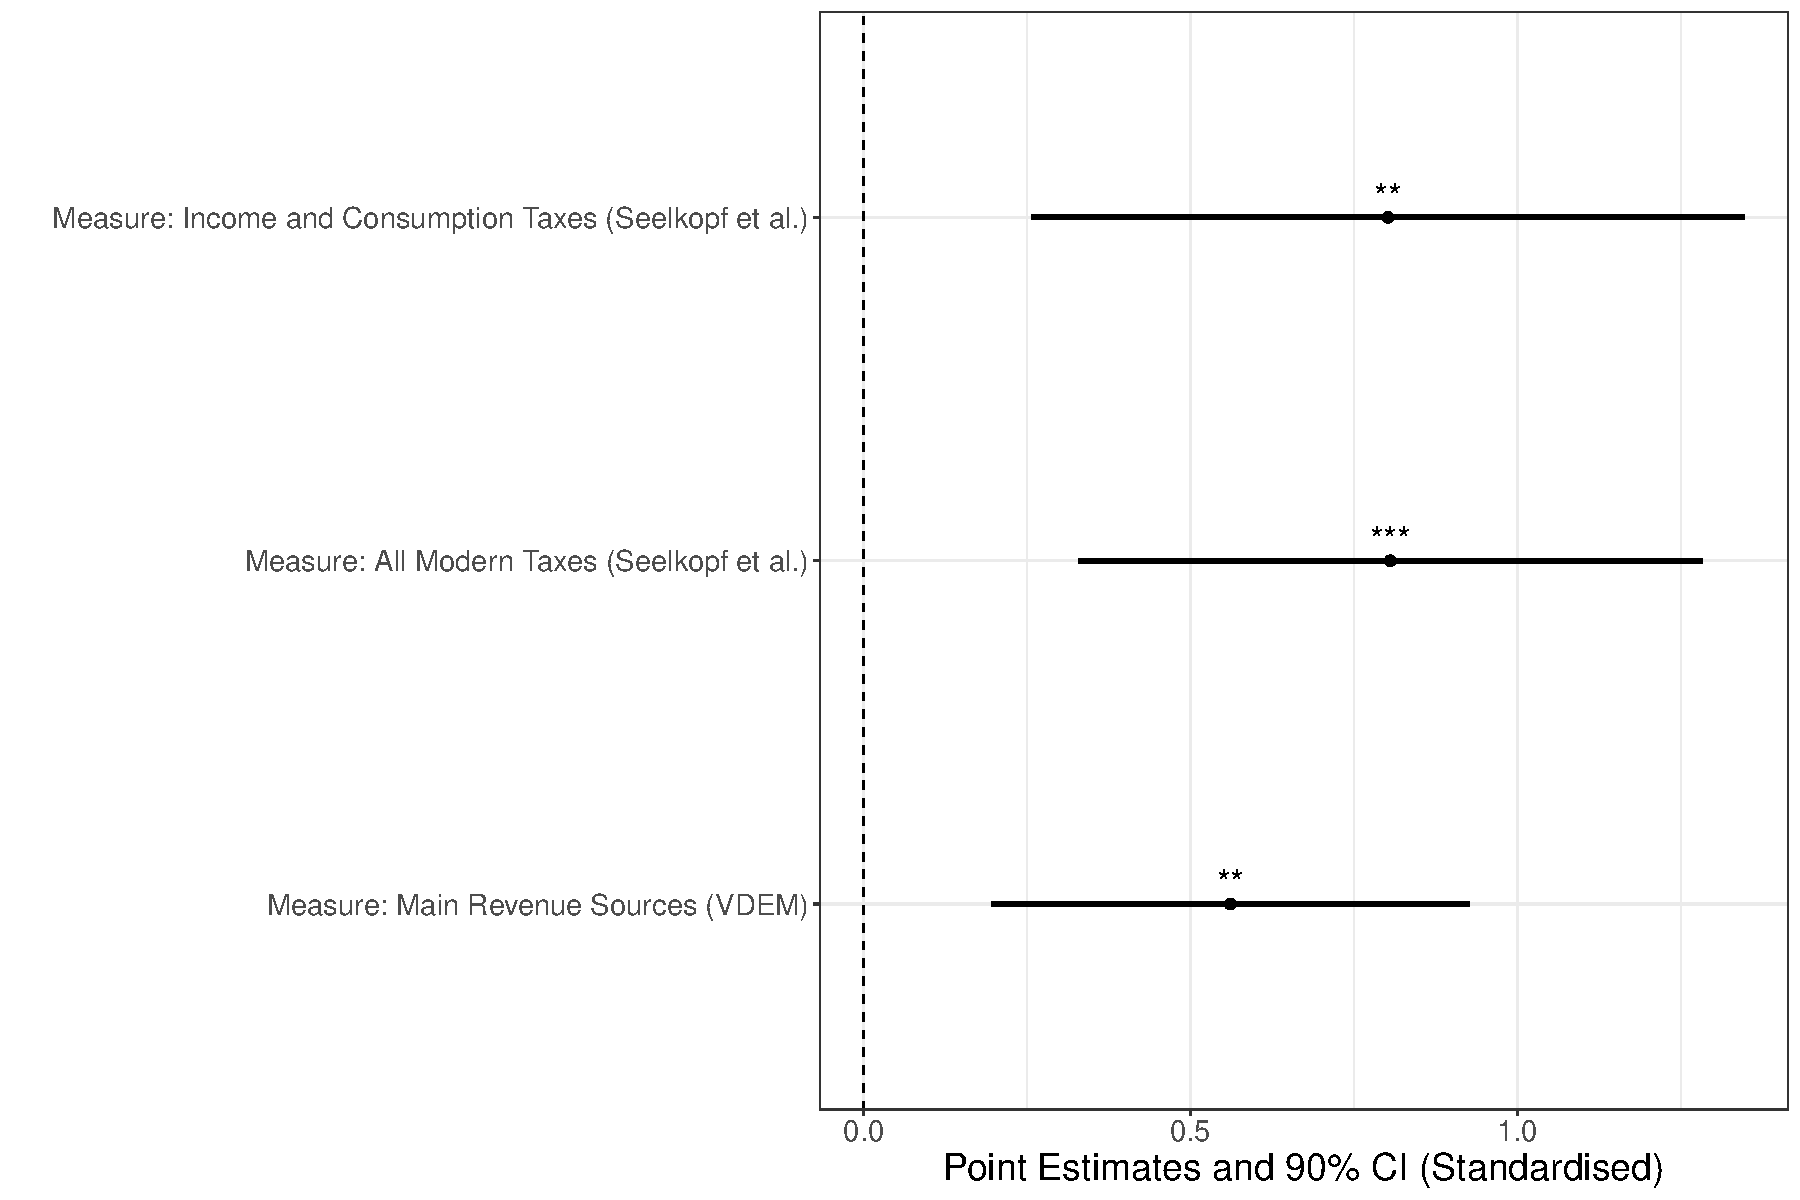
\includegraphics[width=0.7\textwidth]{data_SK/Figure5.pdf}
	\end{figure}
	\begin{figure}[H]\centering
		\caption{Robustness Check: Democracy Measures}
		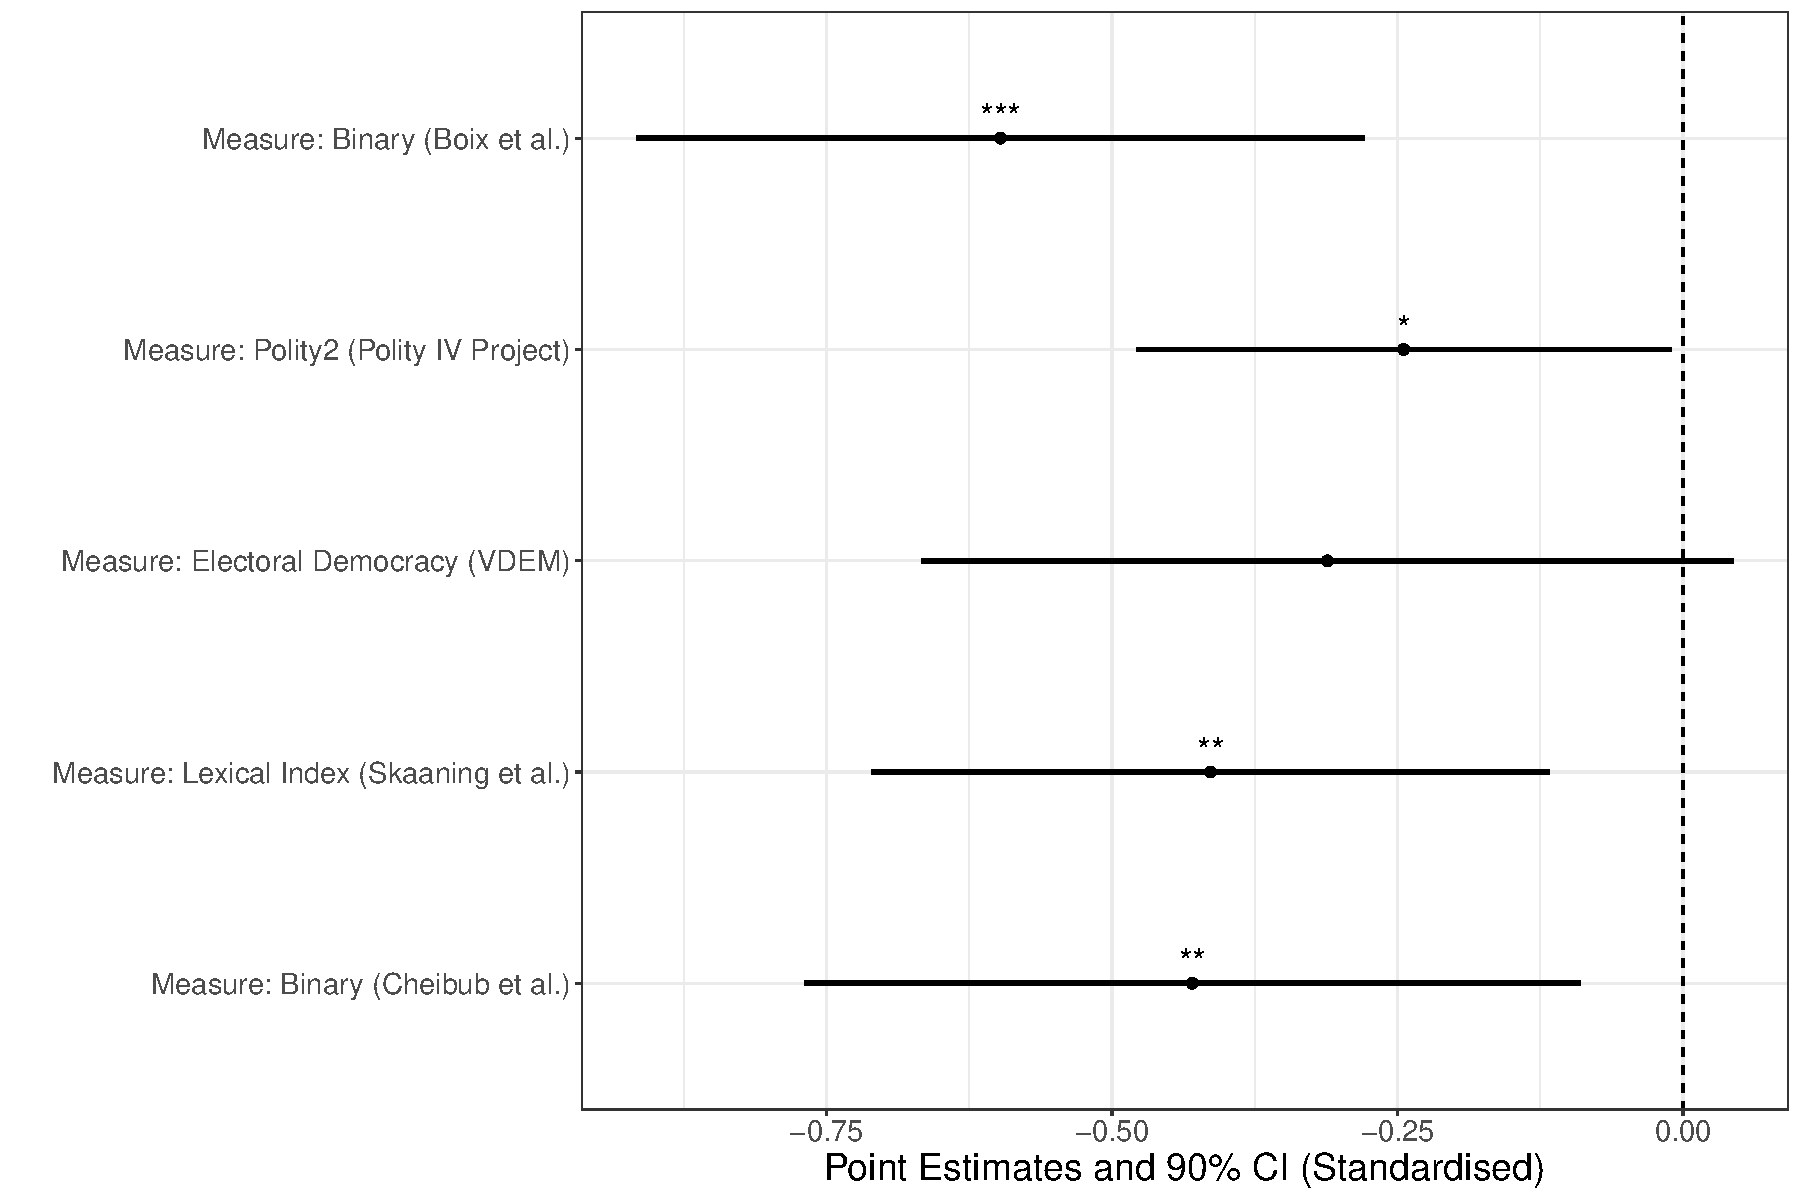
\includegraphics[width=0.7\textwidth]{data_SK/Figure6.pdf}
	\end{figure}
	\noindent According to the authors, the coefficients in these models demonstrate that "the likelihood of inheritance tax repeal increases as governments adopt and expand more efficient revenue instruments," while "democracies are less likely to repeal the inheritance tax than autocracies." 
	
	\newpage
	\section{My Contribution}
	\noindent While the original model provides valuable insights, it is hard to substantively interpret each coefficient.
	For example, if I interpret the coefficient for "Major modern taxes" (1.098) in Table 1: In comparison to not having modern taxes, for each unit increase in the modern tax index, the log-odds of repealing the inheritance tax increase by 1.098 on average, while holding all other variables constant. 
	This log-odds interpretation tells us the direction and statistical significance, but it is not intuitive enough to grasp the actual probability of repeal in real-world scenarios. 
	Moreover, the original model assumes that the effect of modern taxes and the effect of democracy are strictly independent and additive. It ignores the theoretical possibility that democratic institutions might actively moderate the fiscal pressure to repeal the tax. 
	Therefore, in this section, I provide a more intuitive and nuanced interpretation by combining a logistic regression model with an interaction term and predicted probability S-curves. 
	
	\subsection{The Interaction Hypothesis}
	\noindent I argue that we can formulate a theoretical interaction hypothesis:
	\begin{hypothesis} 
		The impact of modern taxes on the likelihood of inheritance tax repeal varies depending on the level of democracy. 
	\end{hypothesis}
	\noindent According to the authors, democracies resist inheritance tax repeals because they protect the redistributive interests of the lower classes. If this is true, even when a state achieves "revenue redundancy" by adopting efficient modern taxes, democratic institutions should resist the fiscal pressure to repeal the inheritance tax more strongly than autocracies. Therefore, the positive effect of the \texttt{other\_tax} variable should be weaker in democratic regimes. 
	
	\subsection{Statistical Concept Application and Visualization}
	To test this hypothesis, I apply the concepts learned in Applied Stats II by adding an interaction term \texttt{(other\_tax * democracy)} to the original logistic regression model. Furthermore, to move beyond the unintuitive log-odds interpretation, I use the \texttt{marginaleffects} package in R. By plotting the predicted probability S-curves, I visually demonstrate how the probability of an inheritance tax repeal behaves differently for democracies versus autocracies as the modern tax index increases.
	\subsubsection{Table 2: Interaction Model}
	\begin{lstlisting}[language=R]
		# Fit interaction model: other_tax * democracy
		model_int <- glm(y ~ other_tax * democracy + war_previous + 
		recession_prev_5 + wfs_intro_previous + 
		log(time_since_intro) + log_gdp_cap + e_pelifeex + 
		log(population_new) + t + t2 + t3,
		data = merge_full_2, family = binomial(link = "logit"))
	\end{lstlisting}
	
	\begin{center}
\begin{small}
\begin{longtable}{l@{} D{.}{.}{4.6}@{} D{.}{.}{4.5}@{}}
\caption{Determinants of Inheritance Tax Repeals (Interaction Model)}
\label{table:coefficients}\\
\toprule
 & \multicolumn{1}{c}{Original (Model 3)} & \multicolumn{1}{c}{Interaction Model} \\
\midrule
\endfirsthead
\toprule
 & \multicolumn{1}{c}{Original (Model 3)} & \multicolumn{1}{c}{Interaction Model} \\
\midrule
\endhead
\bottomrule
\endfoot
\bottomrule
\multicolumn{3}{l}{\tiny{$^{***}p<0.01$; $^{**}p<0.05$; $^{*}p<0.1$}}\\
\endlastfoot
Major Modern Taxes                    & 1.098^{**}   & 1.227^{**} \\
                                      & (0.453)      & (0.548)    \\
Democracy                             & -1.197^{***} & -0.429     \\
                                      & (0.387)      & (1.691)    \\
Major Modern Taxes $\times$ Democracy &              & -0.417     \\
                                      &              & (0.899)    \\
War                                   & 0.764        & 0.756      \\
                                      & (1.066)      & (1.066)    \\
Recession                             & 0.384        & 0.382      \\
                                      & (0.356)      & (0.356)    \\
Social Policy Intro                   & -15.311      & -15.318    \\
                                      & (568.308)    & (569.734)  \\
Tax Competition (Population log)      & 0.034        & 0.028      \\
                                      & (0.127)      & (0.127)    \\
Time Since Intro (log)                & -0.415       & -0.430     \\
                                      & (0.348)      & (0.350)    \\
Life Expectancy                       & 0.062^{**}   & 0.061^{**} \\
                                      & (0.025)      & (0.025)    \\
GDP pc (log)                          & -0.117       & -0.111     \\
                                      & (0.277)      & (0.277)    \\
$t^1$                                 & 0.080        & 0.081      \\
                                      & (0.052)      & (0.053)    \\
$t^2$                                 & -0.001^{*}   & -0.001^{*} \\
                                      & (0.001)      & (0.001)    \\
$t^3$                                 & 0.000^{*}    & 0.000^{*}  \\
                                      & (0.000)      & (0.000)    \\
\midrule
AIC                                   & 452.416      & 454.211    \\
BIC                                   & 539.697      & 548.205    \\
Log Likelihood                        & -213.208     & -213.105   \\
Deviance                              & 426.416      & 426.211    \\
Num. obs.                             & 6087         & 6087       \\
\end{longtable}
\end{small}
\end{center}

	\noindent Note: Table 2 shows that the interaction term Major Modern Taxes x Democracy is negative (-0.417), aligning with the direction of the theoretical hypothesis, although it does not achieve statistical significance at conventional levels.
	
	\vspace{0.5cm}
	\subsubsection{Figure 7: Predicted Probability S-Curves}
	\noindent As visualized in Figure 7, when the modern tax index increases, the predicted probability of an inheritance tax repeal rises sharply in autocracies (red line). In contrast, in democratic regimes (blue line), this curve is significantly flattened, remaining below a 0.01 probability even at the highest levels of the modern tax index. 
	
	\begin{lstlisting}[language=R]
		# Generate Predicted Probability S-Curves
		fig7 <- plot_predictions(model_int, condition = c("other_tax", "democracy")) +
		theme_bw() +
		labs(title = "Predicted Probability of Inheritance Tax Repeal",
		x = "Major Modern Taxes Index", y = "Predicted Probability") +
		scale_color_manual(values = c("red", "blue"), labels = c("Autocracy", "Democracy"))
	\end{lstlisting}
	
	\begin{figure}[H]\centering
		\caption{S-Curves for Autocracy vs. Democracy}
		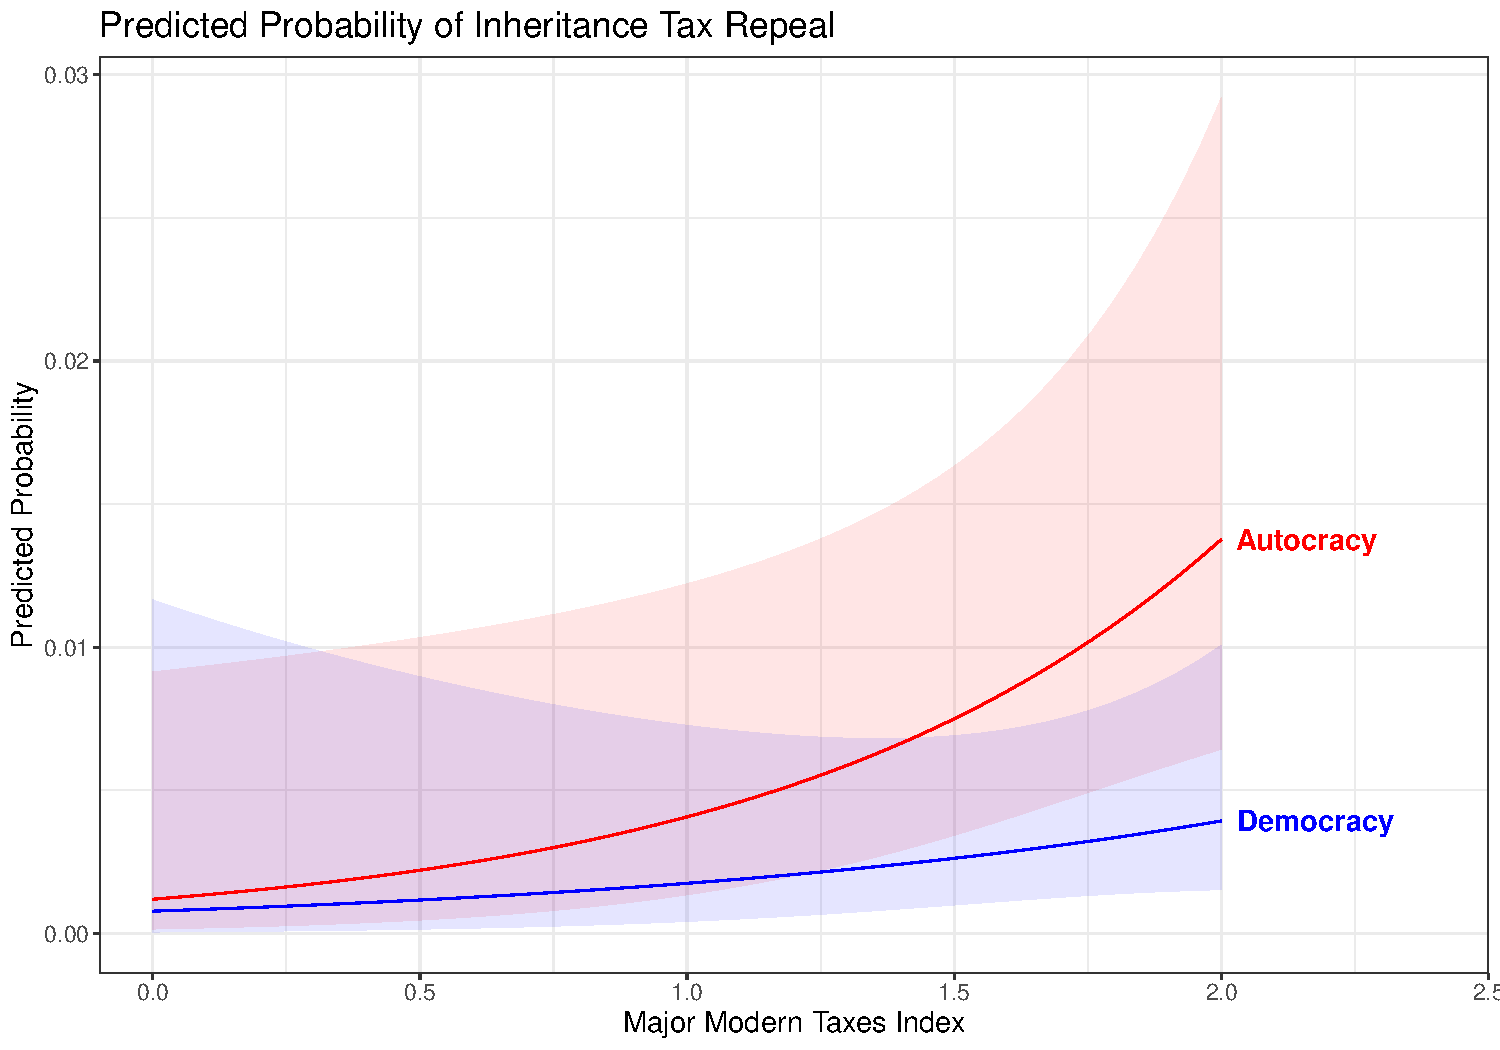
\includegraphics[width=0.7\textwidth]{data_SK/Figure7.pdf}
	\end{figure}
	
	\noindent Although the interaction term itself is not statistically significant—likely due to the overall rarity of repeal events (only 40 out of 6,087 observations)—the graphical representation strongly supports the substantive hypothesis. It effectively demonstrates that democratic institutions serve as a powerful buffer against the fiscal pressures to repeal the inheritance tax, adding a crucial and intuitive nuance to the original authors' additive claims. 
	
\end{document}